\documentclass{article}
\usepackage[preprint]{neurips_2026}
\usepackage[T1]{fontenc}
\usepackage[utf8]{inputenc}
\usepackage{amsmath,amssymb}
\usepackage{booktabs}
\usepackage{graphicx}
\usepackage{url}
\graphicspath{{./}{figures/}{final_results/figures/}}

\title{Do Shallow Graph Neural Networks Improve High-Rating Prediction on MovieLens?}
\author{Lingkai Lei}

\begin{document}
\maketitle

\begin{abstract}
Does a shallow movie-graph neural network improve high-rating prediction over L2 logistic regression on history features? I study preference completion on MovieLens-100K: predict whether an existing user's held-out rating is 4--5 rather than 1--3. Methods share history-only information, eligible targets, and training-only five-fold hyperparameter selection. Thresholds maximize validation precision subject to recall of at least 50\%, then remain fixed. On 9,570 test ratings, logistic regression reaches 80.92\% precision and the original shallow GNN 77.04\%; the paired user-bootstrap difference is $-3.88$ percentage points, with a 95\% interval of $[-5.06,-2.59]$. kNN reaches 81.35\%, without a resolved advantage over logistic regression. Genre features do not clearly help logistic regression and hurt kNN. Three exploratory capacity variants remain below logistic regression. The engineered-history baseline is competitive within this comparison.
\end{abstract}

\section{Introduction}
A useful preference predictor should identify movies a user is likely to rate highly. My question is: \emph{On held-out ratings, does a shallow GNN improve precision over L2 logistic regression on nine history features, at validation-chosen thresholds targeting at least 50\% recall, with a paired user-bootstrap interval excluding zero?} Precision reflects the preference for reliable positive predictions; the recall constraint prevents selecting very few examples.

I compare a movie-rate floor, logistic regression (LR), a kNN classifier, and a shallow movie GNN. Additional experiments add genres to LR/kNN or increase GNN capacity. The original GNN remains the primary comparison; exploratory variants do not replace it. The aim is a fair comparison, not a requirement that graph models win. This is completion of randomly held-out \emph{observed ratings}, not future behavior or recommendation over all unrated movies.

\section{Related work}
\citet{harper2015} document MovieLens and its limitations. Item-based collaborative filtering \citep{sarwar2001} motivates exploiting item similarities; my kNN baseline instead classifies user--movie feature vectors and is not that item-based algorithm. Polynomial graph filtering provides localized graph operations \citep{defferrard2016}. My Lab3-inspired model uses powers of a directed, row-normalized movie adjacency, not that paper's Chebyshev Laplacian filters or pooling. I evaluate this construction rather than the best attainable performance of GNN recommenders.

\clearpage
\section{Data and preprocessing}
MovieLens-100K contains 100,000 integer ratings from 943 users on 1,682 movies, with 19 genre indicators \citep{harper2015}. Data and terms: \url{https://grouplens.org/datasets/movielens/100k/}. IDs align examples; demographic fields are not predictors. Labels are $y=1$ for ratings 4--5 and $y=0$ for 1--3; unobserved pairs are not negatives.

Within each user, approximately 60\% form observed history, 20\% training targets, 10\% validation, and 10\% test. Test/development seeds are 20261106/42. Rounding leaves 61,175 history ratings. Movies absent from history are ineligible, excluding 48/21/26 training/validation/test targets and leaving 19,585/9,575/9,570 rows. Test covers all 943 users; 5,249 ratings (54.85\%) are positive. Flagging every test example has precision 54.85\% and recall 100\%; a constant score has AP 0.5485. This descriptive reference differs from the movie-rate floor.

Rating-derived inputs and the graph use observed history only. Nine baseline features comprise user mean rating/high-rating fraction/count, movie mean rating/high-rating fraction/count, and the user's similarity-weighted mean rating/high-rating fraction/observed-neighbor count around the target. Cosine similarity uses zero-filled history rating columns and at most 20 positive neighbors per movie, without self-edges. With no observed neighbor, weighted statistics revert to the user's history statistics. Targets never enter history. History may postdate a randomly held-out target, so this is preference completion, not chronological forecasting.

\section{Methods}
\paragraph{Course baselines.}
The movie-rate floor scores a movie by its history high-rating fraction. LR uses standardized nine-feature inputs and L2 regularization, selecting $C\in\{.001,.01,.1,1,10,100\}$. kNN uses Euclidean distance with uniform or inverse-distance voting. The final grid is $k\in\{5,15,31,63,127,255,511,1023\}$ for both representations. Every scaler is fitted only on its current training fold. Five-fold mean AP selects pipelines, which are refitted on eligible training targets. LR selects $C=.1$; kNN selects $k=511$, distance voting.

\paragraph{Shallow movie GNN.}
Let $S$ be the movie adjacency, with incoming cosine weights row-normalized. For user $u$, $H_u^{(0)}$ contains history rating divided by 5 and its observation mask. The model is
\begin{equation}
H_u^{(1)}=\operatorname{ReLU}\!\left(\sum_{q=0}^{K-1}S^qH_u^{(0)}W_q+\mathbf{1}b^\top\right),
\qquad s_{ui}=\sigma\!\left((H_u^{(1)})_{i,:}w+c\right).
\label{eq:gnn}
\end{equation}
Weights are shared across users/movies; there are no learned ID embeddings. The hidden layer has 32 channels. Training-only CV chooses $K\in\{3,5\}$ and epochs $\{20,40\}$, selecting $K=5$, 40 epochs (385 parameters). Caching history polynomial signals before gathering targets is equivalent to this one nonlinear graph layer, not a substitution of the nine baseline features.

\paragraph{Genre and capacity experiments.}
LR/kNN gain 57 columns: 19 movie genres, 19 user history genre-specific high-rating rates, and 19 elementwise interactions. Missing genre history reverts to the user's overall history high-rating rate. Original columns remain unchanged. The same CV/grids select genre LR $C=.01$ and genre kNN $k=127$, distance voting. Exploratory GNNs use one layer with 64 or 128 channels ($K=5$; 769/1,537 parameters), or two 32-channel graph layers ($K=3$ each; 3,361 parameters). The second layer propagates learned hidden signals. All have maximum four-hop support and select 40 epochs. These capacity comparisons are exploratory.

\section{Experimental setup}
Fitted models share stratified five-fold training-target assignments (seed 42), selected by mean held-out-fold AP, then refitted on training targets only. History stays fixed across folds; fold-held-out target labels enter neither features nor graph. GNNs minimize binary cross-entropy using Adam (learning rate .005, weight decay .0001, batch size 256, gradient clipping norm 10, seed 20261125). LR/kNN run on CPU; GNNs use an RTX 5080 and PyTorch 2.9.1/CUDA 12.8.

Validation selects the threshold maximizing precision subject to recall $\geq .5$; ties favor higher recall, then higher threshold. Thresholds remain fixed on test, where recall may fall below .5. I report pooled rating-level precision, recall, and average precision (AP). AP summarizes ranking across thresholds, not classification accuracy. The primary effect is $\Delta P=P_{\mathrm{original\ GNN}}-P_{\mathrm{LR}}$.

\paragraph{Model selection and test isolation.}
All reported model configurations, fitted weights, scalers, and decision thresholds are fixed before the reported test evaluation. Hyperparameters are selected by five-fold CV within the training targets; decision thresholds are selected using validation only. Each fitted model in the reported comparison is evaluated once on the same test targets using the same fixed evaluation rules. Test scores are used solely to estimate final performance and paired differences, not to select models, tune hyperparameters, change thresholds, or choose between training runs. Every prespecified method is reported rather than selecting only favorable test results.

I use 2,000 paired user-bootstrap replicates (seed 20261108), resampling users with replacement and retaining all their test ratings. Identical user multiplicities apply to every model. Percentile 95\% intervals summarize metrics and differences, conditional on fitted models/thresholds; they omit training, split, and selection variability. A difference interval crossing zero is inconclusive, not equivalence. Secondary/exploratory intervals are unadjusted for multiple comparisons.

\section{Results}
Table~\ref{tab:test} reports final test performance. Original GNN precision is 77.04\% versus LR's 80.92\%: $\Delta P=-3.88$ percentage points (pp), 95\% CI $[-5.06,-2.59]$. The interval supports a decrease, answering the primary question negatively. Original GNN recall is 49.23\%; I keep its validation threshold rather than tune test recall to 50\%.

% All values below come from final_results/paper_results.json.
% BEGIN GENERATED MAIN TABLE
\begin{table}[htbp]
\centering
\resizebox{\linewidth}{!}{%
\begin{tabular}{lccc}
\toprule
Method & Precision (\%) [95\% CI] & Recall (\%) [95\% CI] & AP [95\% CI] \\
\midrule
Movie-rate floor & 73.67 [71.78, 75.61] & 51.08 [49.34, 52.94] & 0.7261 [0.7061, 0.7469] \\
LR & 80.92 [79.53, 82.37] & 50.75 [48.04, 53.37] & 0.8027 [0.7886, 0.8171] \\
kNN (511) & 81.35 [79.92, 82.81] & 50.70 [48.00, 53.26] & 0.8011 [0.7865, 0.8160] \\
Original GNN & 77.04 [75.56, 78.64] & 49.23 [46.27, 52.00] & 0.7690 [0.7531, 0.7848] \\
\midrule
LR + genre & 80.93 [79.58, 82.43] & 50.60 [47.91, 53.13] & 0.8039 [0.7898, 0.8186] \\
kNN + genre (127) & 78.73 [77.28, 80.19] & 50.85 [48.08, 53.63] & 0.7771 [0.7619, 0.7936] \\
\midrule
GNN wide64 & 77.32 [75.85, 78.85] & 49.11 [46.19, 51.87] & 0.7697 [0.7539, 0.7855] \\
GNN wide128 & 77.09 [75.63, 78.62] & 48.90 [45.98, 51.63] & 0.7702 [0.7543, 0.7860] \\
GNN deep2x32 & 78.22 [76.79, 79.68] & 50.90 [48.19, 53.48] & 0.7791 [0.7631, 0.7949] \\
\bottomrule
\end{tabular}%
}
\caption{Final test performance on 9,570 eligible ratings from 943 users. Thresholds are fixed from validation; realized test recall need not reach 50\%. Every interval is a 95\% user-bootstrap percentile interval (2,000 paired resamples), conditional on fitted models/thresholds. The original shallow GNN is primary; wider/deeper variants are exploratory.}
\label{tab:test}
\end{table}
% END GENERATED MAIN TABLE

\begin{figure}[t]
\centering
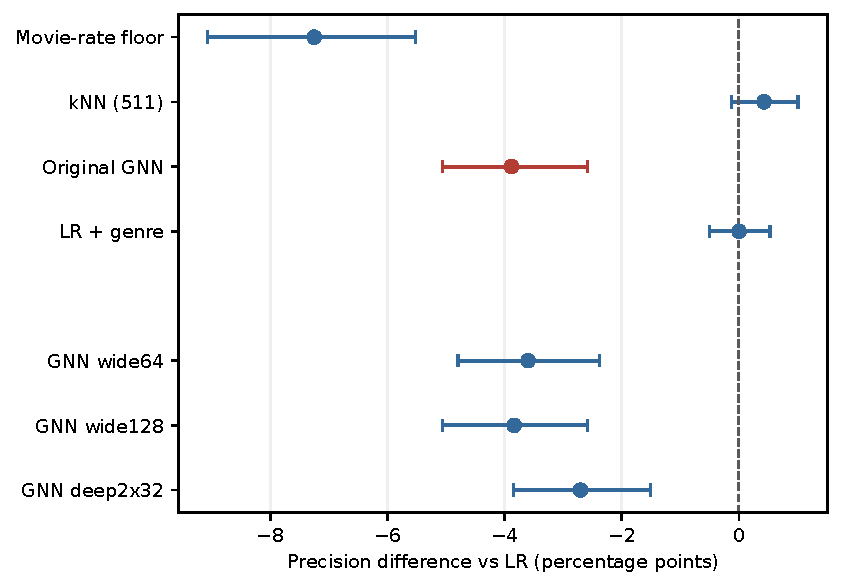
\includegraphics[width=.86\linewidth]{precision_difference_vs_lr.pdf}
\caption{Test precision differences versus LR (percentage points) at frozen validation thresholds. Bars are paired-user 95\% bootstrap intervals; zero marks no difference. Red identifies the original GNN primary comparison. Remaining comparisons are reference, secondary, genre, or exploratory.}
\label{fig:differences}
\end{figure}

kNN reaches 81.35\% precision, but kNN$-$LR is $+0.43$ pp, CI $[-0.12,1.01]$; its AP difference is $-.0016$, CI $[-.0056,.0025]$. Neither resolves an advantage. LR$-$floor precision is $+7.25$ pp, CI $[5.52,9.06]$, supporting this personalized-history pipeline over the movie-only reference. Figure~\ref{fig:differences} shows paired precision intervals; Figure~\ref{fig:pr} shows rankings and fixed-threshold operating points.

Genre$-$history LR precision is $+0.003$ pp, CI $[-0.51,0.53]$, and AP difference $+.0012$, CI $[-.0014,.0038]$: no clear gain. For kNN, genre$-$history precision is $-2.62$ pp, CI $[-3.60,-1.67]$, and AP difference $-.0240$, CI $[-.0313,-.0161]$, supporting a decline despite separate CV tuning.

\begin{figure}[t]
\centering
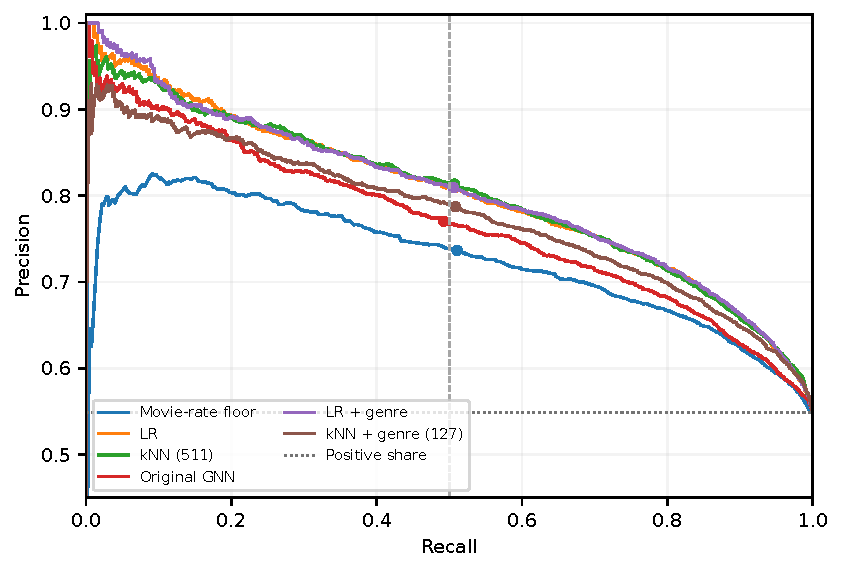
\includegraphics[width=.86\linewidth]{pr_main_models.pdf}
\caption{Test precision--recall curves for baselines, original GNN, genre variants, and movie-rate floor. Dots mark validation-selected thresholds. The vertical recall-.5 line is a reference, not a test tuning rule; the horizontal line is positive prevalence. LR/kNN curves are close; original GNN and genre kNN rank less well.}
\label{fig:pr}
\end{figure}

Against original GNN, wide64 changes precision by $+0.28$ pp, CI $[0.01,0.56]$; wide128 by $+0.04$ pp, CI $[-0.26,0.36]$; and deep2x32 by $+1.18$ pp, CI $[0.43,1.90]$. The first/third unadjusted intervals exclude zero; wide128 is inconclusive. Deep2x32 improves AP by $.0101$, CI $[.0073,.0129]$, but remains below LR in precision ($-2.70$ pp, CI $[-3.85,-1.52]$) and AP ($-.0236$, CI $[-.0310,-.0163]$). This does not show that increasing depth/width generally helps. Appendix~\ref{app:paired} gives all paired comparisons.

\section{Discussion and limitations}
Engineered-history LR is competitive, and graph capacity does not reverse the primary result. However, shared information sources do not mean identical representations: nine summaries versus graph-filtered history. Differences do not isolate a causal effect of graph structure. The deep variant changes parameter count, nonlinearity, and taps as well as depth. Search spaces and tuning budgets also differ across model classes. No experiment establishes over-smoothing as the cause of its performance.

I use one dataset/split, existing users, and movies present in history. Selection of already rated pairs limits conclusions about full-catalog recommendation, cold start, and online satisfaction. History may postdate targets. Folds share users and history, matching the existing-user task rather than new-user generalization. User bootstrap retains within-user dependence but not all cross-user/item dependence or selection uncertainty. Validation thresholds may be optimistic, and exploratory comparisons are unadjusted. The same test set was evaluated previously; it was not used for hyperparameter tuning or threshold selection, and its reuse does not provide independent confirmation.

Numerical reproducibility has limits: two-layer GNN training can vary slightly because of CUDA sparse-matrix operations, even with deterministic settings. All methods here use the same saved graph and inputs.

\section{Conclusion}
The original shallow GNN does not improve high-rating precision over nine-feature L2 logistic regression under this MovieLens-100K protocol. kNN has no resolved advantage over LR; genres do not clearly help LR and hurt this kNN representation. Exploratory GNN extensions improve some metrics over original GNN but remain below LR. These conclusions concern the evaluated pipelines, not all graph recommenders.

\newpage
\paragraph{Code availability and reproducibility.}
I completed this project individually, with no teammates. The repository provides code, configurations, and a README linking step-by-step instructions for preprocessing, training, frozen evaluation, and figure generation: \url{https://github.com/Alko028/ESE5420-MovieLens}. Raw data and user-level outputs are not redistributed.

\section*{Acknowledgments}
I acknowledge GroupLens and the University of Minnesota for MovieLens-100K; use implies no endorsement and raw data are not redistributed. I am the sole author, responsible for the research ideas, final experimental design, interpretation of results, and the main manuscript. OpenAI Codex generated and implemented the project code under my direction and assisted with debugging, experiment execution/checks, figures, literature lookup, and manuscript drafting/editing. I retain responsibility for verifying all AI-assisted outputs and for the final submission.

\clearpage
\begin{thebibliography}{9}
\bibitem[Harper and Konstan(2015)]{harper2015}
F. Maxwell Harper and Joseph A. Konstan.
The MovieLens datasets: History and context.
\emph{ACM Transactions on Interactive Intelligent Systems}, 5(4), Article 19, 2015.
\url{https://doi.org/10.1145/2827872}.

\bibitem[Sarwar et~al.(2001)]{sarwar2001}
Badrul Sarwar, George Karypis, Joseph Konstan, and John Riedl.
Item-based collaborative filtering recommendation algorithms.
In \emph{Proceedings of the 10th International Conference on World Wide Web}, pp.\ 285--295, 2001.
\url{https://files.grouplens.org/papers/www10_sarwar.pdf}.

\bibitem[Defferrard et~al.(2016)]{defferrard2016}
Micha\"el Defferrard, Xavier Bresson, and Pierre Vandergheynst.
Convolutional neural networks on graphs with fast localized spectral filtering.
In \emph{Advances in Neural Information Processing Systems}, volume 29, 2016.
\url{https://arxiv.org/abs/1606.09375}.
\end{thebibliography}

\clearpage
\appendix
\section{Feature and implementation details}
For user $u$ and genre $g$, let $n_{ug}$ count history movies of genre $g$ and $h_{ug}$ count those rated at least four. Preference $p_{ug}=h_{ug}/n_{ug}$ when $n_{ug}>0$, otherwise it is the user's overall history high-rating rate. With target genre vector $g_i$, the three added blocks are $g_i$, $p_u$, and $g_i\odot p_u$. Multi-genre movies contribute once to each indicated genre, including the unknown field. All 66 columns receive fold-local scaling.

For each user's $N_u$ ratings, test/validation each get $\lfloor N_u/10\rfloor$ and training targets $\lfloor N_u/5\rfloor$; history receives the remainder. Filtering is common across methods. Similarity ties nominally favor smaller movie IDs; the saved graph is authoritative across numerical-library changes. Nine-feature neighborhoods use unnormalized cosine weights; GNN inputs additionally row-normalize incoming weights. No target ratings enter either construction.

LR uses L-BFGS (3,000 iterations maximum, tolerance $10^{-6}$). Exact CV ties favor smaller $C$; kNN favors smaller $k$, then uniform voting. Original GNN favors fewer taps, then fewer epochs; capacity variants favor fewer epochs. CV fold $f$ uses seed $20261125+f$ ($f=0,\ldots,4$), final fitting 20261125. Deep2x32 applies a second $K=3$ filter/ReLU over hidden signals for all movies before gathering logits. Loss uses current-fold fit targets only. Its architecture adapts a GNN-course recommendation Lab3; this project's binary objective, splits, and evaluation are separate from the lab experiment.

Implementation checks cover row/label/fold alignment, history-derived inputs, restored models, and independent metric/bootstrap calculations. Figures and tables use saved final evaluation results. No independent human replication was performed for this solo project.

\section{Complete paired comparisons}
\label{app:paired}
The primary endpoint is original GNN minus LR precision. Other comparisons retain secondary/reference/genre/exploratory roles. Precision/recall differences use percentage points; AP differences use the original 0--1 scale. Entries give estimates and paired-user 95\% intervals. LR is the course-baseline reference for the primary and secondary comparisons.

% BEGIN GENERATED PAIRED TABLE
\begin{table}[htbp]
\centering
\resizebox{\linewidth}{!}{%
\begin{tabular}{lccc}
\toprule
Comparison & $\Delta$Precision (pp) & $\Delta$Recall (pp) & $\Delta$AP \\
\midrule
Original GNN $-$ LR & -3.88 [-5.06, -2.59] & -1.52 [-3.56, +0.52] & -0.0337 [-0.0417, -0.0260] \\
kNN (511) $-$ LR & +0.43 [-0.12, +1.01] & -0.06 [-0.78, +0.75] & -0.0016 [-0.0056, +0.0025] \\
LR + genre $-$ LR & +0.00 [-0.51, +0.53] & -0.15 [-0.85, +0.55] & +0.0012 [-0.0014, +0.0038] \\
kNN + genre (127) $-$ kNN (511) & -2.62 [-3.60, -1.67] & +0.15 [-1.07, +1.44] & -0.0240 [-0.0313, -0.0161] \\
Movie-rate floor $-$ LR & -7.25 [-9.06, -5.52] & +0.32 [-2.37, +2.92] & -0.0766 [-0.0921, -0.0614] \\
GNN wide64 $-$ Original GNN & +0.28 [+0.01, +0.56] & -0.11 [-0.43, +0.19] & +0.0007 [+0.0002, +0.0012] \\
GNN wide64 $-$ LR & -3.60 [-4.79, -2.38] & -1.64 [-3.61, +0.33] & -0.0330 [-0.0409, -0.0254] \\
GNN wide128 $-$ Original GNN & +0.04 [-0.26, +0.36] & -0.32 [-0.65, +0.00] & +0.0012 [+0.0006, +0.0018] \\
GNN wide128 $-$ LR & -3.84 [-5.06, -2.59] & -1.85 [-3.85, +0.15] & -0.0325 [-0.0404, -0.0249] \\
GNN deep2x32 $-$ Original GNN & +1.18 [+0.43, +1.90] & +1.68 [+0.65, +2.77] & +0.0101 [+0.0073, +0.0129] \\
GNN deep2x32 $-$ LR & -2.70 [-3.85, -1.52] & +0.15 [-1.60, +1.93] & -0.0236 [-0.0310, -0.0163] \\
\bottomrule
\end{tabular}%
}
\caption{All 11 fixed paired comparisons on the final test results. Original GNN minus LR precision is primary. Other intervals have no multiplicity correction. Positive differences favor the left-hand method.}
\label{tab:all_pairs}
\end{table}
% END GENERATED PAIRED TABLE

\begin{figure}[t]
\centering
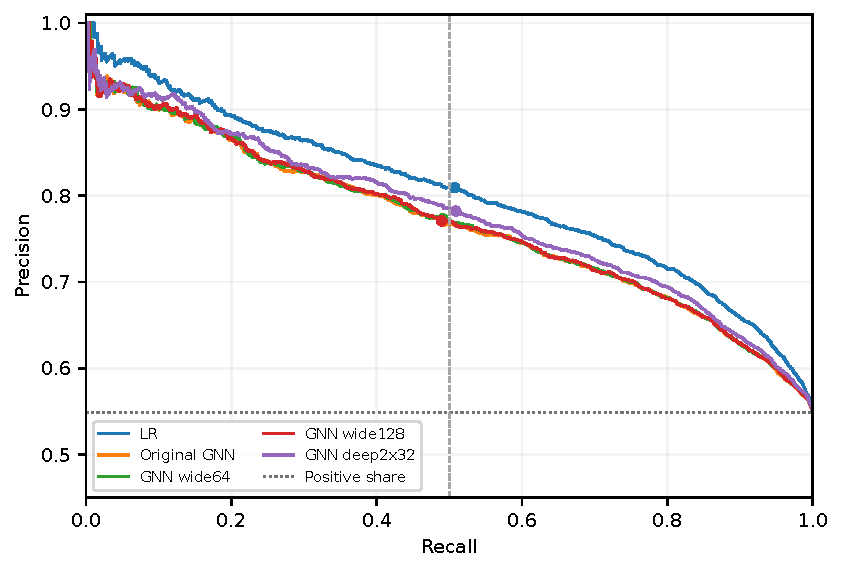
\includegraphics[width=.86\linewidth]{pr_gnn_capacity.pdf}
\caption{Exploratory GNN capacity variants and the LR baseline on identical test ratings. Dots use frozen validation thresholds; the horizontal reference is positive prevalence. Deep2x32 improves ranking over original GNN but stays below LR. These unadjusted comparisons do not isolate depth from parameter count and taps.}
\label{fig:capacity}
\end{figure}

\end{document}
